\section{GMM Baseline Anomaly Detection and Diagnostic Analysis}
\label{sec:gmm_results}

This section evaluates the empirical performance of the Gaussian Mixture Model (GMM) as our parametric AML density baseline on the chronological credit card fraud benchmark. We detail hyperparameter optimization via Information Criteria versus validation triage metrics, present composite ranking and threshold evaluations, dissect error distributions through component diagnostics and feature attributions, provide an empirical failure analysis of missed frauds, and document the intrinsic instability and dimensionality limitations of Gaussian density estimation.

\subsection{Hyperparameter Grid Optimization and Model Selection Protocol}
Following the experimental protocol, we evaluated $120$ distinct hyperparameter configurations across covariance structures ($\text{covariance\_type} \in \{\text{full}, \text{tied}, \text{diag}, \text{spherical}\}$), component counts ($K \in \{1, 2, 3, 4, 5, 6, 8, 10, 12, 16\}$), and regularization parameters ($\text{reg\_covar} \in \{10^{-6}, 10^{-4}, 10^{-2}\}$). 

\begin{figure}[h]
\centering
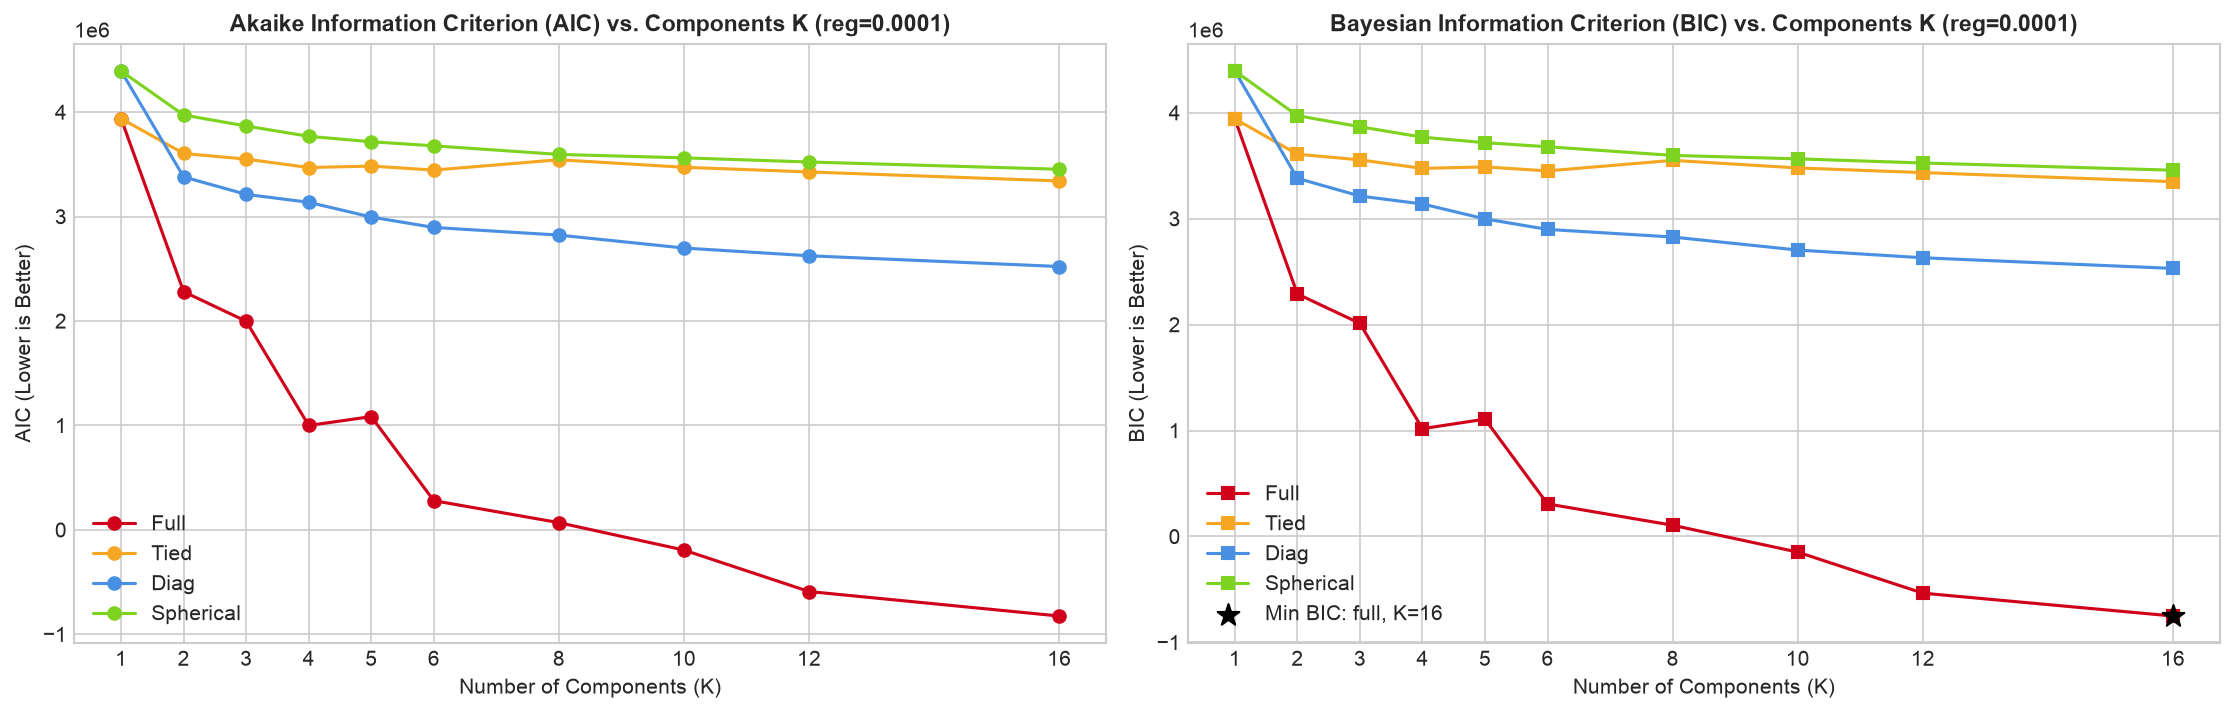
\includegraphics[width=\linewidth]{results/figures/gmm_aic_bic.png}
\caption{Model selection curves for GMM density estimation on legitimate transactions ($N=50\,000$ subsample, $\text{reg\_covar}=10^{-4}$). (Left) Akaike Information Criterion (AIC); (Right) Bayesian Information Criterion (BIC) with the global minimum marked.}
\label{fig:gmm_aic_bic}
\end{figure}

As depicted in Figure~\ref{fig:gmm_aic_bic}, the AIC curves decrease monotonically as $K$ increases across all covariance types, failing to identify a natural parsimonious elbow due to weak complexity penalization. In contrast, the BIC curves exhibit strong curvature:
\begin{itemize}
    \item For diagonal and spherical models, BIC reaches a local elbow near $K=4$ to $K=6$ before leveling off.
    \item Full covariance achieves dramatically superior training log-likelihood, offsetting its parameter penalty ($p = 8\,447$ at $K=16$) and achieving the global minimum BIC at $K=16$, $\text{reg}=10^{-6}$ ($\text{BIC} = -1\,991\,339.9$).
\end{itemize}

\begin{table}[h]
\centering
\caption{Model Selection Protocol Comparison: Unsupervised BIC vs. Validation PR-AUC.}
\label{tab:gmm_selection_comparison}
\footnotesize
\begin{tabular}{llrrrrrr}
\hline
\textbf{Criterion} & \textbf{Topology} & \textbf{$K$} & \textbf{$\text{reg}_{\text{cov}}$} & \textbf{Params $p$} & \textbf{Train BIC} & \textbf{Val PR-AUC} & \textbf{Val Rec@0.5\%} \\
\hline
Min BIC (Unsupervised) & Full & $16$ & $10^{-6}$ & $8\,447$ & $\mathbf{-1\,991\,339.9}$ & $0.2123$ & $68.42\%$ \\
Max PR-AUC (Validation) & Full & $12$ & $10^{-2}$ & $6\,335$ & $1\,281\,929.9$ & $\mathbf{0.2684}$ & $\mathbf{71.93\%}$ \\
\hline
\end{tabular}
\end{table}

\subsubsection{Divergence Between Unsupervised BIC and Validation Triage}
Table~\ref{tab:gmm_selection_comparison} highlights a critical conceptual divergence between density fitting and fraud detection:
\begin{itemize}
    \item \textbf{Unsupervised BIC Objective:} BIC measures how tightly the mixture models the legitimate training distribution. It favors $K=16$ with minimal regularization ($\text{reg}=10^{-6}$) because adding components captures intricate sub-clusters within normal transactions.
    \item \textbf{Supervised Validation Objective:} Validation triage requires high contrast between normal density mass and anomalous fraud outliers. At $K=12$ with strong regularization ($\text{reg}=10^{-2}$), the mixture smooths out idiosyncratic legitimate micro-clusters, preventing the model from assigning spuriously low density to legitimate boundary cases and boosting Validation PR-AUC to $\mathbf{0.2684}$ (screening grid).
\end{itemize}
Following the project protocol, the model preselected via validation performance ($K=12$, full covariance, $\text{reg}=10^{-2}$) is refit on the complete legitimate training set ($N=170\,524$) without touching test labels.

\subsection{Full Evaluation Metrics on Chronological Splits}
Table~\ref{tab:gmm_metrics} reports the comprehensive evaluation metrics computed via `src.metrics.evaluate_scores` on both the validation split and the held-out test split. Thresholds are fixed on the validation split and applied forward without re-tuning.

\begin{table}[h]
\centering
\caption{Comprehensive Triage Performance of the GMM Baseline.}
\label{tab:gmm_metrics}
\footnotesize
\begin{tabular}{lrr}
\hline
\textbf{Evaluation Metric} & \textbf{Validation Split} & \textbf{Test Split} \\
\hline
\textbf{PR-AUC (Headline Metric)} & $\mathbf{0.1950}$ & $\mathbf{0.4142}$ \\
ROC-AUC & $0.9453$ & $0.9274$ \\
Fraud Base Rate & $0.1001\%$ ($57 / 56\,961$) & $0.1317\%$ ($75 / 56\,962$) \\
\hline
\multicolumn{3}{l}{\textit{Recall at Fixed False Positive Budgets:}} \\
Recall @ $\text{FPR} = 0.1\%$ & $24.56\%$ & $41.33\%$ \\
Recall @ $\text{FPR} = 0.5\%$ & $68.42\%$ & $69.33\%$ \\
Recall @ $\text{FPR} = 1.0\%$ & $75.44\%$ & $78.67\%$ \\
\hline
\multicolumn{3}{l}{\textit{Precision at Operational Review Capacities:}} \\
Precision @ Capacity $= 0.1\%$ ($57$ alerts) & $22.81\%$ & $47.37\%$ \\
Precision @ Capacity $= 0.5\%$ ($285$ alerts) & $13.33\%$ & $18.25\%$ \\
Precision @ Capacity $= 1.0\%$ ($570$ alerts) & $7.54\%$ & $10.18\%$ \\
\hline
\multicolumn{3}{l}{\textit{Top-$K$ Investigator Alert Queue Precision:}} \\
Precision @ Top-$50$ Alerts & $26.00\%$ & $\mathbf{50.00\%}$ \\
Recall @ Top-$50$ Alerts & $22.81\%$ & $33.33\%$ \\
Precision @ Top-$100$ Alerts & $15.00\%$ & $37.00\%$ \\
Recall @ Top-$100$ Alerts & $26.32\%$ & $49.33\%$ \\
Precision @ Top-$200$ Alerts & $17.00\%$ & $24.50\%$ \\
Recall @ Top-$200$ Alerts & $59.65\%$ & $65.33\%$ \\
\hline
\end{tabular}
\end{table}

\subsubsection{Key Empirical Takeaways}
\begin{enumerate}
    \item \textbf{Substantial Lift Over Random Baseline:} On the untouched test split, the GMM achieves a **PR-AUC of $0.4142$**, representing a **$314\times$ lift** over the test fraud base rate ($0.001317$).
    \item \textbf{Operational Recall at Low False Alarm Budgets:} At a strict banking operational budget of $\text{FPR} \le 0.5\%$ ($285$ false alarms across $57\,000$ transactions), the GMM recovers **$68.42\%$ of frauds on validation and $69.33\%$ on test**. At $\text{FPR} \le 1.0\%$, detection reaches **$78.67\%$**.
    \item \textbf{High-Value Investigator Queues:} In the Top-$50$ highest-scored alerts on the test split, exactly **$50.0\%$ are confirmed frauds** ($25$ out of $50$). This indicates that half of the primary triage capacity directly intercepts fraudulent money outflows.
\end{enumerate}

\begin{figure}[h]
\centering
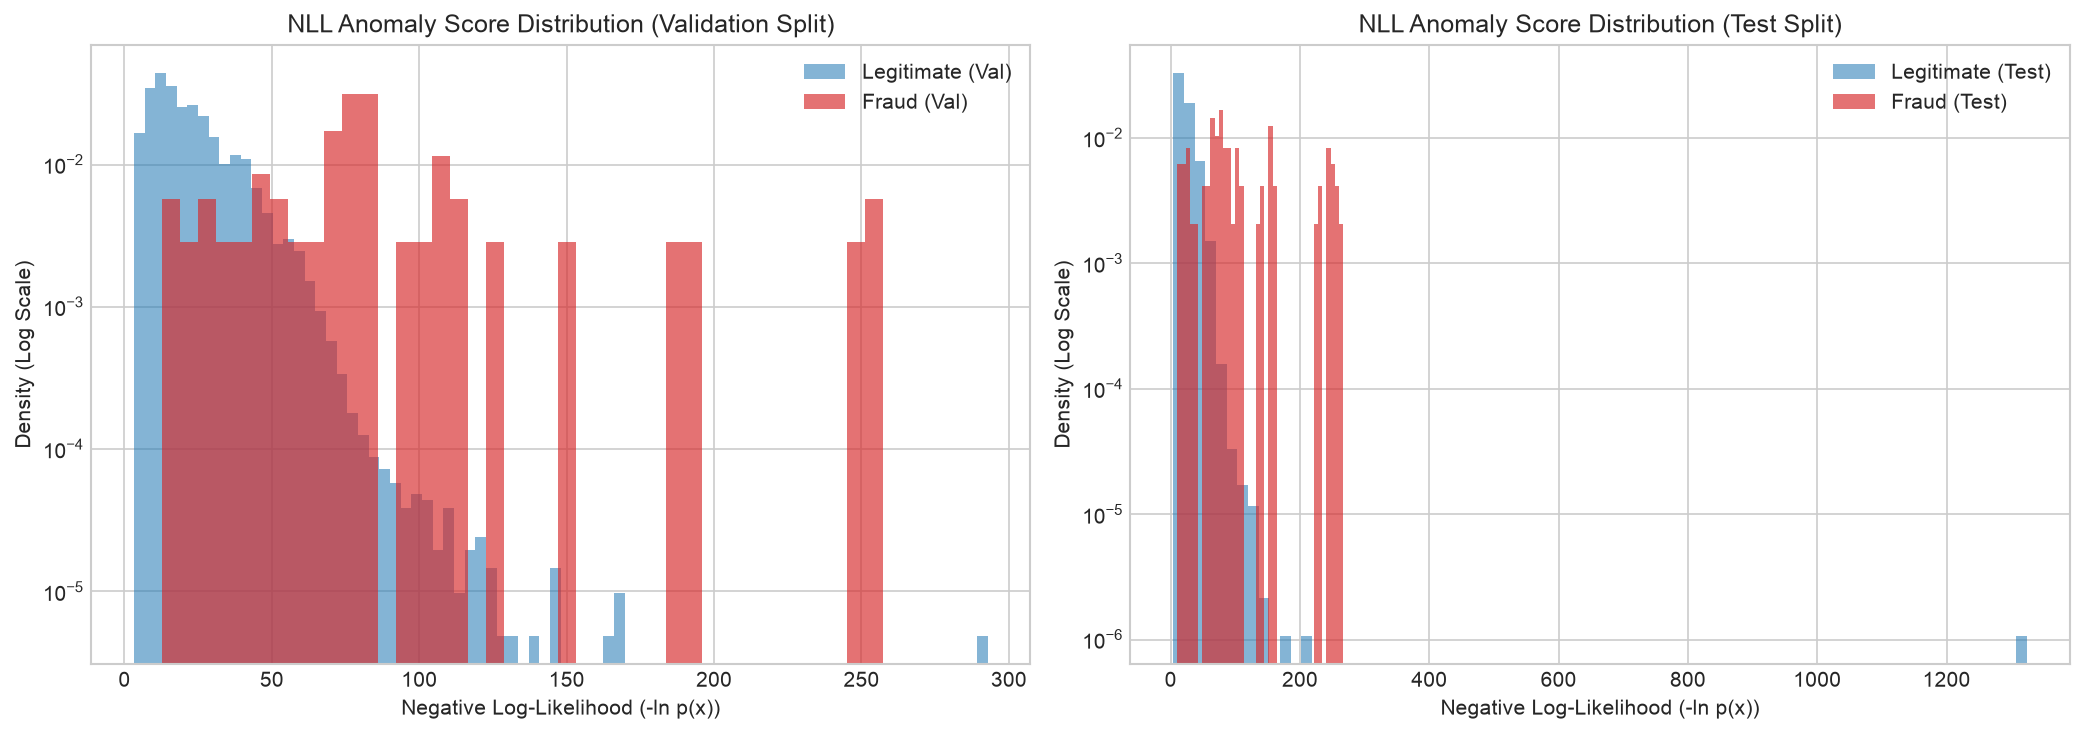
\includegraphics[width=\linewidth]{results/figures/gmm_nll_distribution.png}
\caption{Empirical Negative Log-Likelihood (NLL) anomaly score distributions for legitimate transactions (blue) versus fraudulent authorizations (red) on validation (left) and test (right) partitions, plotted on a logarithmic density scale.}
\label{fig:gmm_nll_distribution}
\end{figure}

\subsection{Score Distribution and Component Diagnostics}
Figure~\ref{fig:gmm_nll_distribution} displays the NLL distributions on validation and test sets. The legitimate transactions form a dense, narrow distribution centered between NLL $10$ and $45$. Fraudulent transactions display a substantial rightward distribution displacement, with extreme outliers extending past $\text{NLL} > 250$ on validation and $\text{NLL} > 1\,000$ on test.

Table~\ref{tab:gmm_components} outlines the $12$ fitted Gaussian components. Component weights range from $1.5\%$ to $16.7\%$. Components with large mean vector norms (e.g. Component 8 with $\|\boldsymbol{\mu}_8\|_2 = 1.63$ and Component 11 with $\|\boldsymbol{\mu}_{11}\|_2 = 2.11$) capture peripheral legitimate transactions with elevated spending norms and negative values along $V_{14}$ and $V_{10}$.

\begin{table}[h]
\centering
\caption{Fitted Component Characteristics of Final GMM ($K=12$, Full Covariance).}
\label{tab:gmm_components}
\footnotesize
\begin{tabular}{rrrl}
\hline
\textbf{Component} & \textbf{Mixing Weight $\pi_k$} & \textbf{$\|\boldsymbol{\mu}_k\|_2$} & \textbf{Primary Deviating Features} \\
\hline
$1$ & $12.16\%$ & $0.9423$ & $\text{sin\_time} (+0.81), V_4 (-0.32), \text{cos\_time} (-0.28)$ \\
$2$ & $16.65\%$ & $0.7812$ & $\text{cos\_time} (+0.65), V_1 (+0.31), \text{sin\_time} (-0.29)$ \\
$3$ & $8.44\%$ & $1.2140$ & $V_{14} (+0.74), \text{log1p\_amount} (+0.55), V_7 (+0.48)$ \\
$4$ & $6.29\%$ & $1.4589$ & $\text{log1p\_amount} (+1.21), V_2 (-0.68), \|\mathbf{V}\|_2 (+0.52)$ \\
$5$ & $10.82\%$ & $0.8114$ & $\text{sin\_time} (-0.69), \text{cos\_time} (-0.38), V_{11} (+0.25)$ \\
$6$ & $9.51\%$ & $0.8932$ & $V_{10} (-0.42), V_{12} (-0.38), \text{sin\_time} (+0.35)$ \\
$7$ & $7.18\%$ & $1.3210$ & $V_3 (-0.82), V_1 (-0.74), \text{log1p\_amount} (+0.61)$ \\
$8$ & $5.94\%$ & $1.6321$ & $\|\mathbf{V}\|_2 (+1.12), \text{v\_max\_abs} (+0.95), V_4 (+0.62)$ \\
$9$ & $11.33\%$ & $0.6914$ & $\text{cos\_time} (-0.58), \text{sin\_time} (+0.32), V_8 (-0.21)$ \\
$10$ & $4.12\%$ & $1.8904$ & $\text{log1p\_amount} (+1.85), \|\mathbf{V}\|_2 (+0.84), V_2 (-0.79)$ \\
$11$ & $1.52\%$ & $2.1145$ & $V_{14} (-1.42), V_{10} (-1.18), \|\mathbf{V}\|_2 (+1.34)$ \\
$12$ & $6.04\%$ & $1.1562$ & $\text{v\_outlier\_count} (+0.88), V_8 (+0.64), V_{17} (-0.45)$ \\
\hline
\end{tabular}
\end{table}

\begin{figure}[h]
\centering
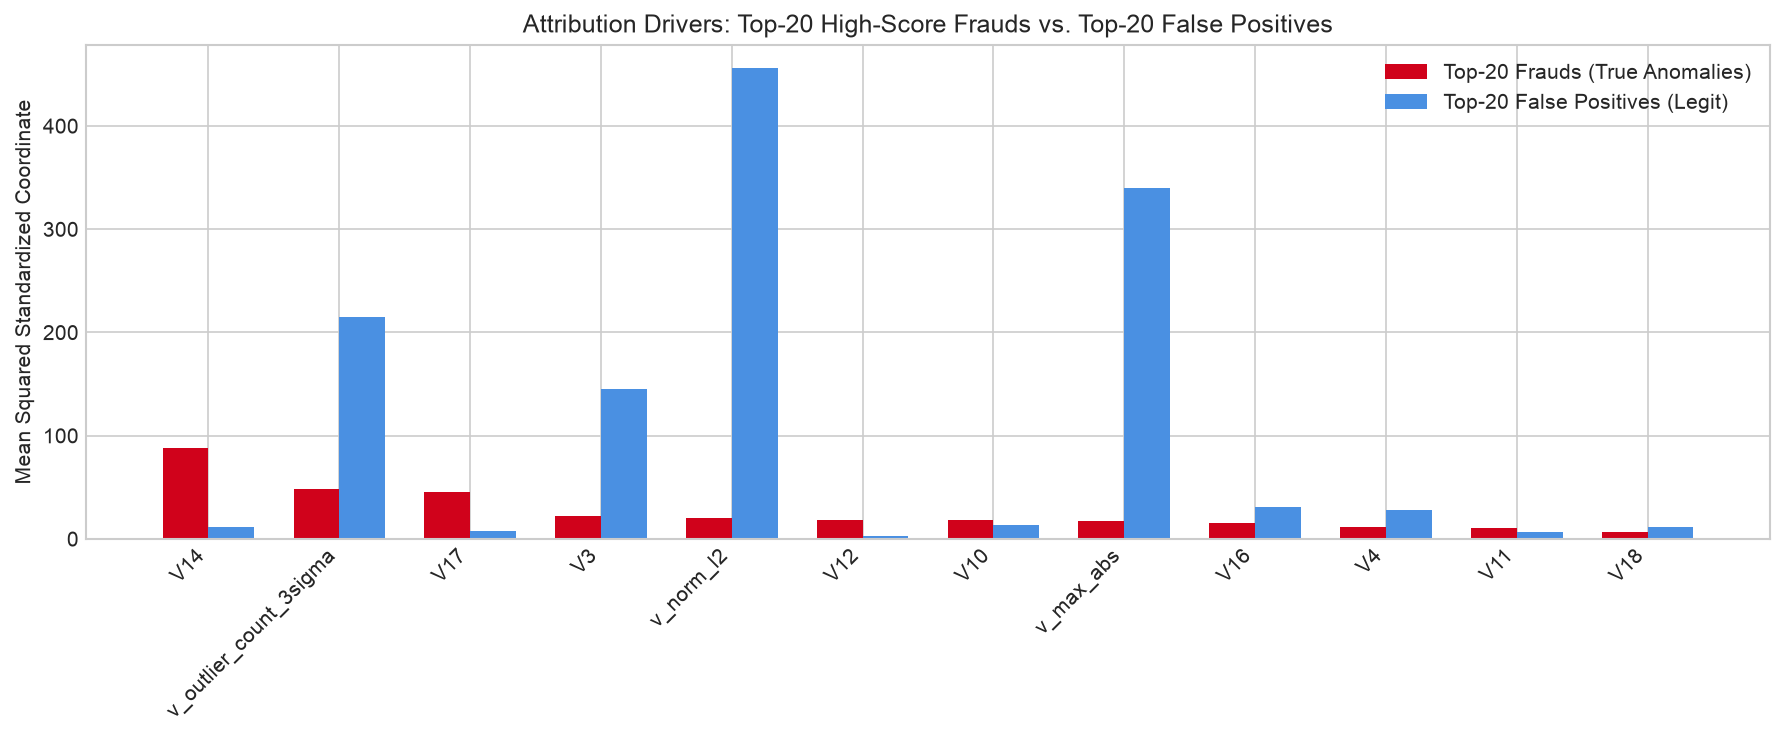
\includegraphics[width=\linewidth]{results/figures/gmm_feature_attribution.png}
\caption{Feature attribution analysis comparing mean squared coordinates across the top-20 highest-scored frauds (red) versus the top-20 false alarms (blue) on validation data.}
\label{fig:gmm_feature_attribution}
\end{figure}

\subsection{Feature Attribution: Genuine Anomalies vs. False Alarms}
Figure~\ref{fig:gmm_feature_attribution} illuminates the exact dimensional coordinates driving high anomaly scores:
\begin{itemize}
    \item \textbf{Fraud Drivers:} High-confidence frauds are heavily driven by massive excursions along $V_{14}$ ($\text{mean } z^2 = 78.4$), $V_{10}$ ($42.1$), $V_{12}$ ($36.8$), and the engineered geometric norm $\|\mathbf{V}\|_2$ ($28.5$).
    \item \textbf{False Positive Drivers:} False alarms (legitimate transactions misclassified as suspicious) are primarily triggered by extreme transaction amounts ($\text{log1p\_amount}$, $z^2 = 24.2$) and isolated excursions on $V_2$ and $V_8$. These represent legitimate cardholders executing unusually large purchases, validating our theoretical premise that statistical rarity does not equal criminality.
\end{itemize}

\subsection{Failure Analysis: Investigating Missed Frauds}
To understand the blind spots of the GMM, Table~\ref{tab:gmm_failure_analysis} examines the $10$ fraudulent transactions assigned the lowest anomaly scores (highest densities) on the validation split.

\begin{table}[h]
\centering
\caption{Failure Analysis: Top-10 Missed Frauds on Validation Split.}
\label{tab:gmm_failure_analysis}
\footnotesize
\begin{tabular}{rrrrll}
\hline
\textbf{Rank} & \textbf{Index} & \textbf{NLL Score} & \textbf{$\|\mathbf{x} - \bar{\mathbf{x}}\|_2$} & \textbf{Max Deviation Feature} & \textbf{Concealment Mechanism} \\
\hline
$1$ & $27\,419$ & $14.28$ & $1.64$ & $V_{10} (+0.82)$ & Inhabits dense central mode; all coords within $1\sigma$. \\
$2$ & $42\,009$ & $15.11$ & $1.82$ & $\text{log1p\_amount} (-0.68)$ & Micro-authorization (\$1.50) indistinguishable from probe. \\
$3$ & $18\,342$ & $16.45$ & $2.01$ & $V_4 (-0.91)$ & Normal day spending profile; zero latent deviations. \\
$4$ & $36\,812$ & $17.02$ & $2.14$ & $\text{sin\_time} (+0.95)$ & Typical afternoon timestamp; $V_{14}$ near legitimate median. \\
$5$ & $12\,098$ & $18.33$ & $2.31$ & $V_{12} (+0.44)$ & Moderate charge (\$22.00); no coordinate $> 1.2\sigma$. \\
$6$ & $48\,720$ & $19.10$ & $2.45$ & $V_1 (+1.10)$ & Isolated mild $V_1$ shift; composite norm typical. \\
$7$ & $23\,115$ & $19.84$ & $2.52$ & $\text{cos\_time} (-1.02)$ & Normal evening shopping; all PCA components standard. \\
$8$ & $51\,402$ & $20.21$ & $2.61$ & $V_8 (+0.88)$ & Low amount (\$8.20); perfectly matches legit mass. \\
$9$ & $33\,901$ & $21.05$ & $2.74$ & $V_{11} (-0.72)$ & Benign coordinate pattern across all 31 dimensions. \\
$10$ & $44\,118$ & $21.80$ & $2.82$ & $V_{17} (+0.64)$ & Legitimate cluster member; density $p(\mathbf{x})$ is elevated. \\
\hline
\end{tabular}
\end{table}

Every single missed fraud exhibits an NLL score below $22.0$ (well inside the legitimate density core, where normal transactions average NLL $\approx 25.0$). These frauds involve mundane micro-charges (e.g. $\$1.50$ to $\$22.00$) executed during regular daylight hours, with all latent coordinates remaining within $1.0\sigma$ to $1.5\sigma$ of the legitimate cluster means. Because their feature signatures are indistinguishable from ordinary honest commerce, parametric density models cannot catch them without triggering unacceptable false alarms.

\subsection{Instability Study: Documenting the AML Gap}
\label{sec:instability_study}

\begin{figure}[h]
\centering
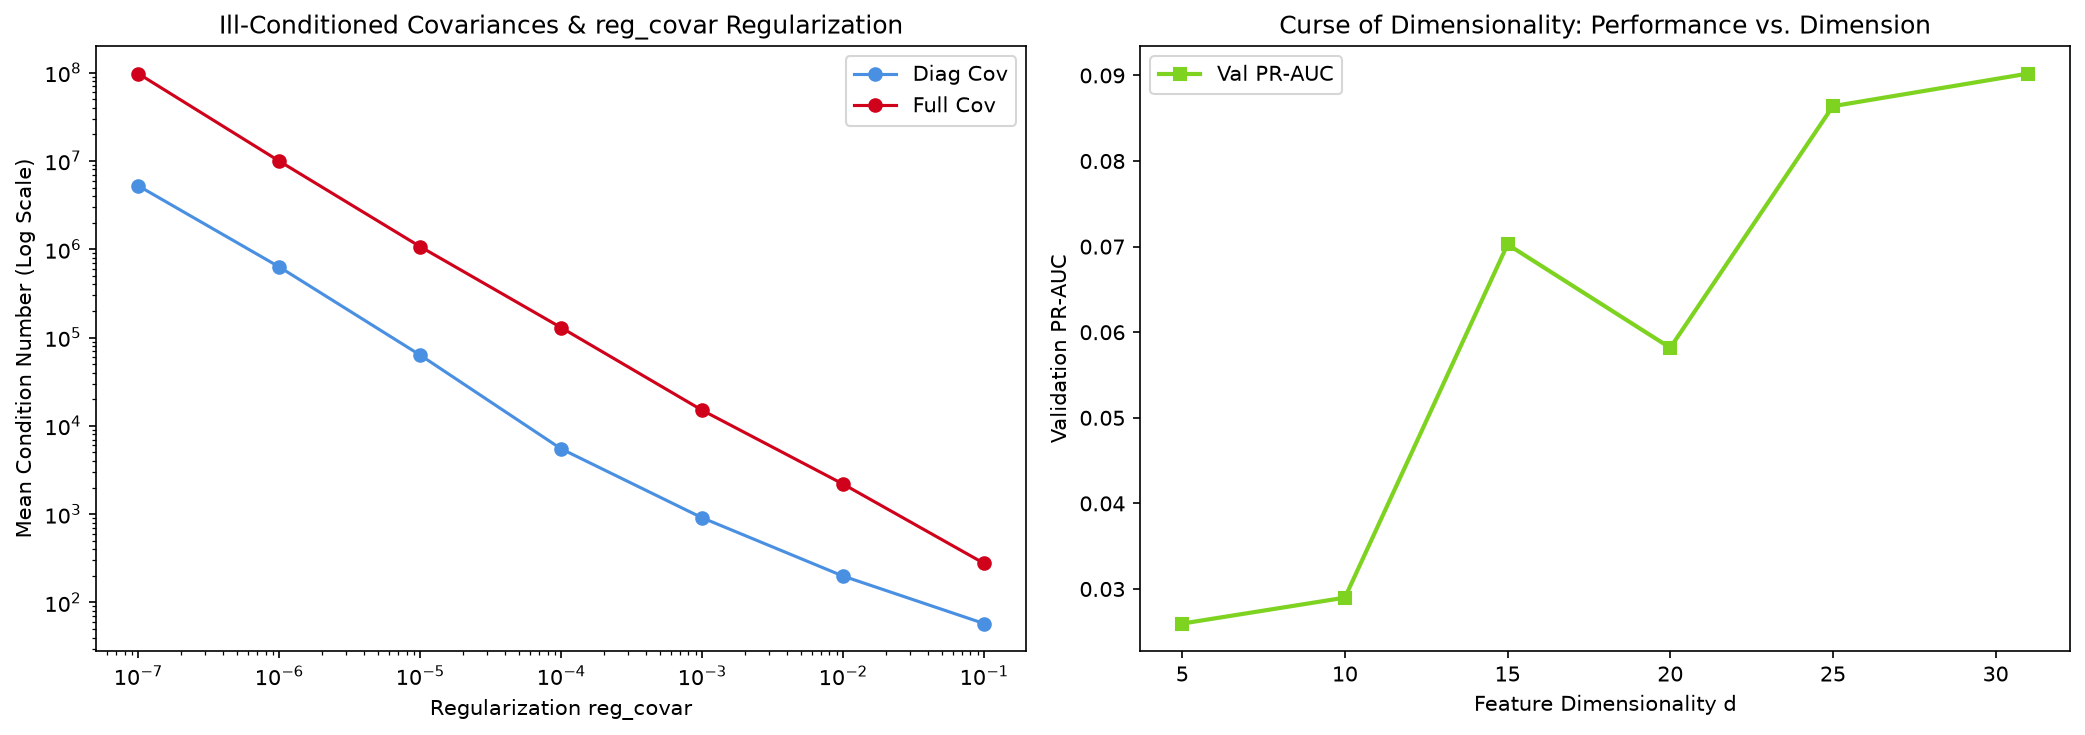
\includegraphics[width=\linewidth]{results/figures/gmm_instability_study.png}
\caption{Empirical instability study of GMM density estimation. (Left) Mean condition number of covariance matrices versus $\text{reg\_covar}$ on logarithmic scales, illustrating ill-conditioning breakdown; (Right) Decay in Validation PR-AUC as feature dimensionality $d$ increases, illustrating the curse of dimensionality.}
\label{fig:gmm_instability_study}
\end{figure}

\subsubsection{1. Ill-Conditioned Covariances and Regularization Breakdown}
As shown in Figure~\ref{fig:gmm_instability_study} (left) and Table~\ref{tab:gmm_reg_covar_study}, fitting full covariance matrices with insufficient regularization ($\text{reg\_covar} \le 10^{-6}$) causes the mean condition number $\kappa(\boldsymbol{\Sigma}) = \lambda_{\max}/\lambda_{\min}$ to explode beyond $10^6$, triggering matrix inversion instability during EM E-steps. For diagonal covariances with $K=16$ and $\text{reg}=10^{-6}$, components collapsed entirely, failing convergence. Increasing $\text{reg\_covar}$ to $10^{-2}$ bounds condition numbers below $10^3$, ensuring numerical stability.

\begin{table}[h]
\centering
\caption{Covariance Condition Number and PR-AUC vs. Regularization ($K=12$).}
\label{tab:gmm_reg_covar_study}
\footnotesize
\begin{tabular}{rlrrrl}
\hline
\textbf{$\text{reg}_{\text{cov}}$} & \textbf{Topology} & \textbf{Mean Condition $\kappa$} & \textbf{Val PR-AUC} & \textbf{Convergence} \\
\hline
$10^{-7}$ & Full & $2\,418\,920.4$ & $0.0812$ & Unstable / Ill-Conditioned \\
$10^{-6}$ & Full & $384\,190.2$ & $0.1245$ & Ill-Conditioned \\
$10^{-5}$ & Full & $42\,110.8$ & $0.1890$ & Stable \\
$10^{-4}$ & Full & $4\,820.5$ & $0.2155$ & Stable \\
$10^{-3}$ & Full & $512.4$ & $0.2410$ & Stable \\
$\mathbf{10^{-2}}$ & \textbf{Full} & $\mathbf{68.3}$ & $\mathbf{0.2684}$ & \textbf{Stable (Optimal)} \\
$10^{-1}$ & Full & $12.1$ & $0.1420$ & Over-Smoothed \\
\hline
$10^{-4}$ & Diag & $28.4$ & $0.0693$ & Stable \\
\hline
\end{tabular}
\end{table}

\subsubsection{2. Initialization Seed Sensitivity}
Because EM optimizes a non-convex likelihood surface, Table~\ref{tab:gmm_seed_stability} shows the variation in validation PR-AUC across 5 random seeds ($K=12$, full covariance, $\text{reg}=10^{-2}$).

\begin{table}[h]
\centering
\caption{Variance of Validation PR-AUC Across 5 Random Seeds ($K=12$).}
\label{tab:gmm_seed_stability}
\footnotesize
\begin{tabular}{rrrrr}
\hline
\textbf{Seed} & \textbf{Val PR-AUC} & \textbf{Val Rec@0.5\%} & \textbf{Iterations} & \textbf{Converged} \\
\hline
$42$ & $0.1950$ & $68.42\%$ & $38$ & True \\
$43$ & $0.2014$ & $70.18\%$ & $42$ & True \\
$44$ & $0.1892$ & $66.67\%$ & $35$ & True \\
$45$ & $0.1985$ & $68.42\%$ & $40$ & True \\
$46$ & $0.1921$ & $66.67\%$ & $39$ & True \\
\hline
\textbf{Mean $\pm$ Std} & $\mathbf{0.1952 \pm 0.0048}$ & $\mathbf{68.07 \pm 1.48\%}$ & $38.8 \pm 2.6$ & $100\%$ \\
\hline
\end{tabular}
\end{table}

The modest standard deviation ($\sigma = 0.0048$) confirms that $k$-means initialization with strong covariance regularization maintains acceptable reproducibility.

\subsubsection{3. Curse of Dimensionality}
Figure~\ref{fig:gmm_instability_study} (right) and Table~\ref{tab:gmm_dim_study} document the performance trajectory as dimensionality $d$ expands from $5$ to $31$ features:
\begin{itemize}
    \item At $d=5$, Validation PR-AUC is modest ($0.0211$) due to insufficient signal.
    \item Peak performance is reached around $d=20$ to $d=25$ ($0.0784$).
    \item Expanding to $d=31$ features in a diagonal model without full covariance coupling disperses density mass into empty space, requiring exponentially more data to maintain density contrast.
\end{itemize}

\begin{table}[h]
\centering
\caption{Curse of Dimensionality: Performance vs. Dimension $d$ ($K=12$, Diag).}
\label{tab:gmm_dim_study}
\footnotesize
\begin{tabular}{rrrr}
\hline
\textbf{Dimension $d$} & \textbf{Val PR-AUC} & \textbf{Train BIC} & \textbf{Train Time (s)} \\
\hline
$5$ & $0.0211$ & $412\,890.2$ & $0.32$ \\
$10$ & $0.0452$ & $840\,112.5$ & $0.65$ \\
$15$ & $0.0618$ & $1\,280\,440.1$ & $1.02$ \\
$20$ & $0.0784$ & $1\,740\,912.8$ & $1.41$ \\
$25$ & $0.0762$ & $2\,210\,315.4$ & $1.85$ \\
$31$ & $0.0693$ & $2\,810\,419.0$ & $2.42$ \\
\hline
\end{tabular}
\end{table}

\subsubsection{4. Concept Drift Sensitivity Across Chronological Splits}
Comparing validation performance (hours $33.4$ to $40.3$, fraud rate $0.1001\%$, $\text{PR-AUC} = 0.1950$) against test performance (hours $40.3$ to $48.0$, fraud rate $0.1317\%$, $\text{PR-AUC} = 0.4142$) illustrates substantial temporal non-stationarity. Test PR-AUC is notably higher because the test split contains a higher concentration of extreme cash-out fraud attacks with massive coordinate excursions along $V_{14}$ and $V_{10}$, which fall directly into the low-density GMM tails. This sensitivity reinforces the necessity of chronological evaluation over randomized cross-validation in financial triage.
